%% img/complexity_intro/NPCONP.tex
%% Copyright 2019 Andrea Berlingieri
%
% This work may be distributed and/or modified under the
% conditions of the LaTeX Project Public License, either version 1.3
% of this license or (at your option) any later version.
% The latest version of this license is in
%   http://www.latex-project.org/lppl.txt
% and version 1.3 or later is part of all distributions of LaTeX
% version 2005/12/01 or later.
%
% This work has the LPPL maintenance status `maintained'.
%
% The Current Maintainer of this work is Andrea Berlingieri.
%
% This work consists of all files listed in manifest.txt
\documentclass{standalone}
\usepackage{../TikzStyle}
\usepackage{../mystyle}
\usepackage{amsmath}
\usepackage{tikz}
\usepackage{mathdots}
\usepackage{yhmath}
\usepackage{cancel}
\usepackage{color}
\usepackage{siunitx}
\usepackage{array}
\usepackage{multirow}
\usepackage{amssymb}
\usepackage{gensymb}
\usepackage{tabularx}
\usepackage{booktabs}
\usetikzlibrary{fadings}

\begin{document}

\tikzset{every picture/.style={line width=0.75pt}} %set default line width to 0.75pt        

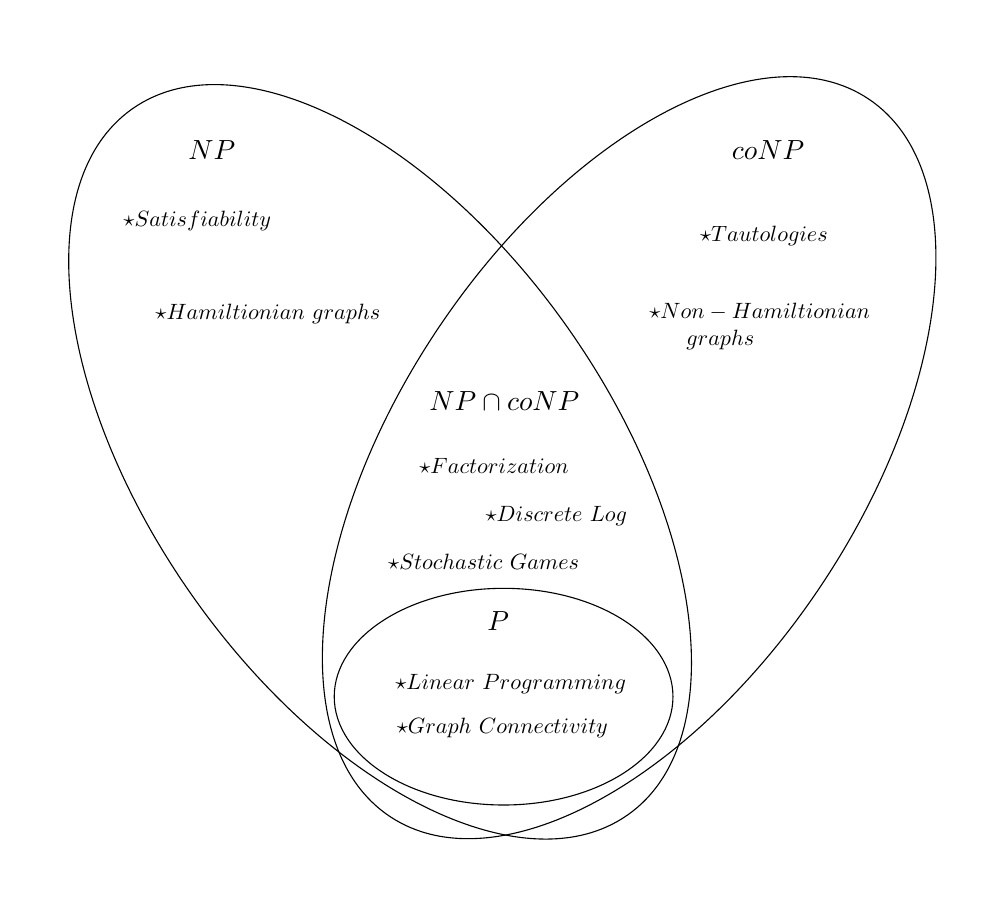
\begin{tikzpicture}[x=0.75pt,y=0.75pt,yscale=-1,xscale=1]
    
    %Shape: Ellipse [id:dp8535738819839966] 
    \draw  [fill={rgb, 255:red, 255; green, 255; blue, 255 }  ,fill opacity=0 ] (256,304.2) .. controls (256,275.37) and (292.53,252) .. (337.6,252) .. controls (382.67,252) and (419.2,275.37) .. (419.2,304.2) .. controls (419.2,333.03) and (382.67,356.4) .. (337.6,356.4) .. controls (292.53,356.4) and (256,333.03) .. (256,304.2) -- cycle ;
    %Shape: Ellipse [id:dp4560276355894095] 
    \draw   (282.77,361.9) .. controls (231.72,327.84) and (241.96,222.84) .. (305.65,127.38) .. controls (369.34,31.92) and (462.35,-17.85) .. (513.41,16.21) .. controls (564.46,50.27) and (554.22,155.27) .. (490.53,250.73) .. controls (426.84,346.19) and (333.83,395.96) .. (282.77,361.9) -- cycle ;
    %Shape: Ellipse [id:dp17371054321509327] 
    \draw   (397.36,361.2) .. controls (347.1,396.43) and (252.97,348.81) .. (187.1,254.84) .. controls (121.23,160.88) and (108.57,56.14) .. (158.82,20.91) .. controls (209.08,-14.31) and (303.21,33.3) .. (369.08,127.27) .. controls (434.95,221.24) and (447.61,325.97) .. (397.36,361.2) -- cycle ;

    % Text Node
    \draw (338,162) node   {$NP\cap coNP$};
    % Text Node
    \draw (197,41) node   {$NP$};
    % Text Node
    \draw (465,41) node   {$coNP$};
    % Text Node
    \draw (190,75) node [scale=0.8]  {$\star Satisfiability$};
    % Text Node
    \draw (224,120) node [scale=0.8]  {$\star Hamiltionian\ graphs$};
    % Text Node
    \draw (463,82) node [scale=0.8]  {$\star Tautologies$};
    % Text Node
    \draw (461,126) node [scale=0.8]  {$ \begin{array}{l}
    \star Non-Hamiltionian\\
    \ \ \ \ \ graphs
    \end{array}$};
    % Text Node
    \draw (341,298.2) node [scale=0.8]  {$\star Linear\ Programming$};
    % Text Node
    \draw (335,268) node   {$P$};
    % Text Node
    \draw (337,319.2) node [scale=0.8]  {$\star Graph\ Connectivity$};
    % Text Node
    \draw (333,193) node [scale=0.8]  {$\star Factorization$};
    % Text Node
    \draw (363,217) node [scale=0.8]  {$\star Discrete\ Log$};
    % Text Node
    \draw (328,239) node [scale=0.8]  {$\star Stochastic\ Games$};
\end{tikzpicture}


\end{document}
